\chapter{Modèles nucléaires}

\section{Introduction}
L'équation de Schrödinger $H\Psi=E\Psi$ d'un noyau ne peut pas être résolue exactement pour $A>4$. Le problème
est le terme potentiel qui - bien qu'il paraît inoffensif - cache une double somme
\begin{equation}
H=\sum_{i=1}^AT_i+\sum_{i>j=1}^A V_{ij}
\end{equation}
où $T_i=\vec{p_i^2}/(2m_N)$ est l'énergie cinétique du nucléon $i$ et $V_{ij}$ l'interaction entre les nucléons
$i$ et $j$.\\

En plus de n'être pas résolvable analytiquement, le potentiel nucléon-nucléon $V_{ij}$ n'est pas exactement 
connu, il existe des forces à 3 corps, 4 corps, \dots ainsi que des effets relativistes difficiles à inclure. Pour
s'en sortir il convient d'utiliser des modèles respectant les principes physiques et reproduisant certaines
propriétés du noyau. Il existe deux classes de modèles
\begin{enumerate}
\item Particules indépendantes : chaque nucléon est pris en compte individuellement
\item Collectifs : le noyau est considéré comme un ensemble
\end{enumerate}


\section{Modèle du gaz de Fermi}
	\begin{wrapfigure}[9]{l}{2.5cm}
	\vspace{-5mm}
	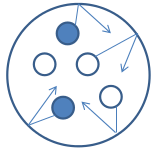
\includegraphics[scale=0.4]{ch8/image1}
	\captionof{figure}{ }
	\end{wrapfigure}
Il s'agit d'un modèle à particules indépendantes
\begin{equation}
\Psi(r_1,r_2,\dots, r_A) = \phi_1(r_1)\phi_2(r_2)\dots\phi_A(r_A)
\end{equation}
Ce modèle considère que les nucléons sont dans une "boîte", dans laquelle ils n'interagissent pas. Ceci est 
décrit par un potentiel de \textit{sphère dure} $V_i(r_i)$
\begin{equation}
V=\sum_{i=1}^A V_i, \qquad\qquad V_i(r_i)=0\ \text{si}\ r\leq a,\qquad\qquad V_i(r_i)=\infty\text{ si }r>a
\end{equation}
Les fonctions individuelles sont celles de particules dans une boîte cubique de côté $a$ 
\begin{equation}
\phi_i(x,y,z) = A\sin(k_xx)\sin(k_yy)\sin(k_zz)
\end{equation}
où $k_xa=n_a\pi,k_ya=n_y\pi$ et $k_za=n_z\pi$. Ce modèle permet d'expliquer certains termes de la formule de 
masse (celui élaboré lors du modèle de la goutte liquide, à savoir le terme de volume et d'asymétrie). 
L'énergie d'individuelle est alors donnée par
\begin{equation}
E(n_x,n_y,n_z) = \frac{a\hbar^2}{2m}(k_x^2+k_y^2+k_z^2) = \frac{\hbar^2k^2}{2m} = \frac{\hbar^2\pi^2}{2ma^2}
(n_x^2+n_y^2+n_z^2)
\end{equation}

\newpage
	\begin{wrapfigure}[11]{r}{5.5cm}
	\vspace{-5mm}
	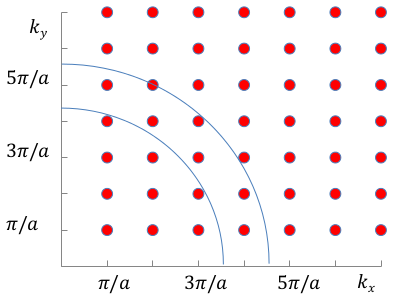
\includegraphics[scale=0.4]{ch8/image2}
	\captionof{figure}{ }
	\end{wrapfigure}
	
Ci-contre, une représentation bidimensionnelle des valeurs d'énergies accessibles pour un nucléon. Chaque état
peut être occupé par maximum quatre nucléons (spin/isospin).Le nombre d'états entre $k$ et $k+dk$ est donné par
\begin{equation}
dn = 4\times 4\pi k^2dk\times\left(\frac{a}{\pi}\right)^3
\end{equation}
où $\pi/a$ est le volume d'une cellule. Dès lors
\begin{equation}
\frac{dn}{dk} = \frac{2}{\pi^2}k^2V
\end{equation}
où $V=a^3$ est le volume du noyau (supposé cubique). Le nombre total de nucléon $A$ doit donc respecter la
relation (l'intégration doit forcément donner le nombre de nucléons)
\begin{equation}
A = \int_0^{k_F} \frac{dn}{dk}dk = \frac{2}{3\pi^2}k_F^2V
\end{equation}
où $\DS k_F = \left(\frac{3\pi^2}{2}\frac{A}{V}\right)^{1/3} = 1.33$ fm$^{-1}$ est le \textbf{nombre d'onde de
Fermi}. Comme la densité $\rho = A/V$ est connue, on peut facilement trouver l'énergie individuelle maximale
dite l'\textbf{énergie de Fermi}
\begin{equation}
\epsilon_F = \frac{\hbar^2k_F^2}{2m_N}=\frac{a\hbar^2}{2m_N}\left(\frac{3\pi^2}{2}\rho\right)^2 \approx
37\ \text{MeV}
\end{equation}


	\begin{wrapfigure}[8]{l}{7.5cm}
	\vspace{-5mm}
	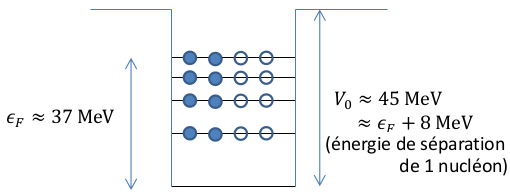
\includegraphics[scale=0.4]{ch8/image3}
	\captionof{figure}{ }
	\end{wrapfigure}
	

Les orbitales sont ainsi remplies jusqu'au niveau de \textsc{Fermi} et il est alors facile, sachant ça, de 
calculer l'énergie totale du noyau en effectuant la somme sur tous les nucléons. 
\begin{equation}
E = \int_0^{k_F} \frac{\hbar^2k^2}{2m_N}dn = \frac{\hbar^2}{2m_N}\frac{2k_F^5}{5\pi^2}V = \frac{3}{5}\epsilon_F
A \approx 22.2\ \text{A}
\end{equation}
On retrouve la forme du terme de volume ($B(Z,A) = a_VA+\dots$). L'énergie est proportionnelle au nombre 
de nucléons ce qui justifie la forme précédemment utilisée.\\



	\begin{wrapfigure}[8]{r}{3cm}
	\vspace{-5mm}
	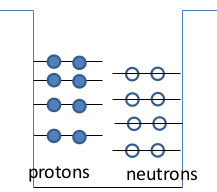
\includegraphics[scale=0.4]{ch8/image4}
	\captionof{figure}{ }
	\end{wrapfigure}
On peut également considérer l'asymétrie neutron-proton en considérant des énergies de \textsc{Fermi} différentes
pour chacune de ces deux espèces\footnote{Si le noyau est asymétrique, l'énergie de liaison diminue.}
\begin{equation}
E_p(Z) = \frac{3}{5}\epsilon_F(p)Z = \frac{\hbar^2}{2m_N}\left(\frac{3\pi^2}{2}\frac{Z}{V}\right)^{2/3}Z
\end{equation}
\begin{equation}
E_n(Z) = \frac{3}{5}\epsilon_F(p)N = \frac{\hbar^2}{2m_N}\left(\frac{3\pi^2}{2}\frac{N}{V}\right)^{2/3}N
\end{equation}
L'énergie d'asymétrie est obtenue en prenant la différence entre deux énergie : l'une qui serait l'énergie 
s'il n'y avait pas de différence entre neutrons et protons et l'autre l'énergie spécifique associée aux 
protons et aux neutrons
\begin{equation}
\Delta E = 2E(A/2)-E(Z)-E(N) = -\frac{1}{3}\epsilon_F\frac{(N-Z)^2}{A}
\end{equation}
On retrouve le terme d'asymétrie dans le modèle de la goutte liquide ($B(A,Z) = \dots - a_a\frac{(N-Z)^2}{A}+
\dots$).\\

\textsc{Conclusions}\\
Ce modèle permet d'expliquer la forme des termes de volume et d'asymétrie (mais pas l'ajustement des 
paramètres). Lorsqu'on s'intéresse aux fonctions d'ondes, dans le modèle de particules indépendantes comme
c'est le cas ici, on obtient un produit de fonctions d'onde individuelles. Celles-ci décrivant des fermions,
il faut que lafonction d'onde soit antisymétrique
\begin{equation}
\Psi(r_1,r_2,\dots, r_A) =\mathcal{A} \phi_1(r_1)\phi_2(r_2)\dots\phi_A(r_A)
\end{equation}
où $A =\sum_{p=1}^{A!} \epsilon_pP_p$ est l'opérateur \textit{anti-symétriseur} avec $P_p$ la permutations de 
$A$ éléments et $\epsilon_p$ le signe de la permutation. Il est possible d'écrire cette fonction d'onde sous
la forme d'un déterminant de \textsc{Slater}.










